\documentclass{article}
\usepackage[a4paper]{geometry}
\usepackage[spanish]{babel}
\usepackage{parskip}
\usepackage{setspace}
\usepackage{graphicx}
\usepackage{typearea}
\usepackage{fancyhdr}
\geometry{total={6in, 9in}}


%HEADRULE

\pagestyle{fancy}
\setlength{\headheight}{30.2pt}
\setlength{\headsep}{30pt}

%INICIO DEL DOCUMENTO   
\begin{document}
\onehalfspacing    
\begin{titlepage}
	
	
	\begin{center}
		{\LARGE \textbf{UNIVERSIDAD NACIONAL DE INGENIERÍA}}\\
		\vspace{5 mm}
		{\LARGE \textbf{Facultad de Ingeniería Industrial y de Sistemas}}\\
		\vspace{6.5 mm}
		\begin{figure}[h]
			\centering 
			
\includegraphics[width=0.4\textwidth]{images/logo-UNI.png}
		\end{figure}
		\vspace{4 mm}	
		{\Large \textbf{Aplicativo para la creación de parejas de gatos} }\\
		\vspace{5 mm}
		
		\onehalfspacing  % Espaciamiento 1.5
		{\Large \textbf{``{\@TinderCat}''} }\\
		
		\singlespacing  % Fin del espaciamiento 1.5
		
		\vspace{4 mm}	

		\vspace{10 mm}
		{\large \textbf{ELABORADO POR:} }\\
		\vspace{10 mm}
		\begin{center}
			\begin{minipage}{0.6\textwidth}
			  \begin{itemize}
				\item \Large Matta Mendoza, Hugo
				\item \Large Mottoccanche Tantaruna, Joseph
				\item \Large Ventocilla Lázaro, Omar
				\item \Large Páucar Del Rosario, Elian
			  \end{itemize}
			\end{minipage}
		  \end{center}

		\vspace{5 mm}	
	\end{center}

\end{titlepage}


\clearpage
\tableofcontents
%--------------------------------------------------------------------------------
\clearpage 
\section{Modelo de Negocio}
\subsection{Caso de uso negocio}
\vspace{5mm}
\begin{figure}[h]
    \begin{center}
        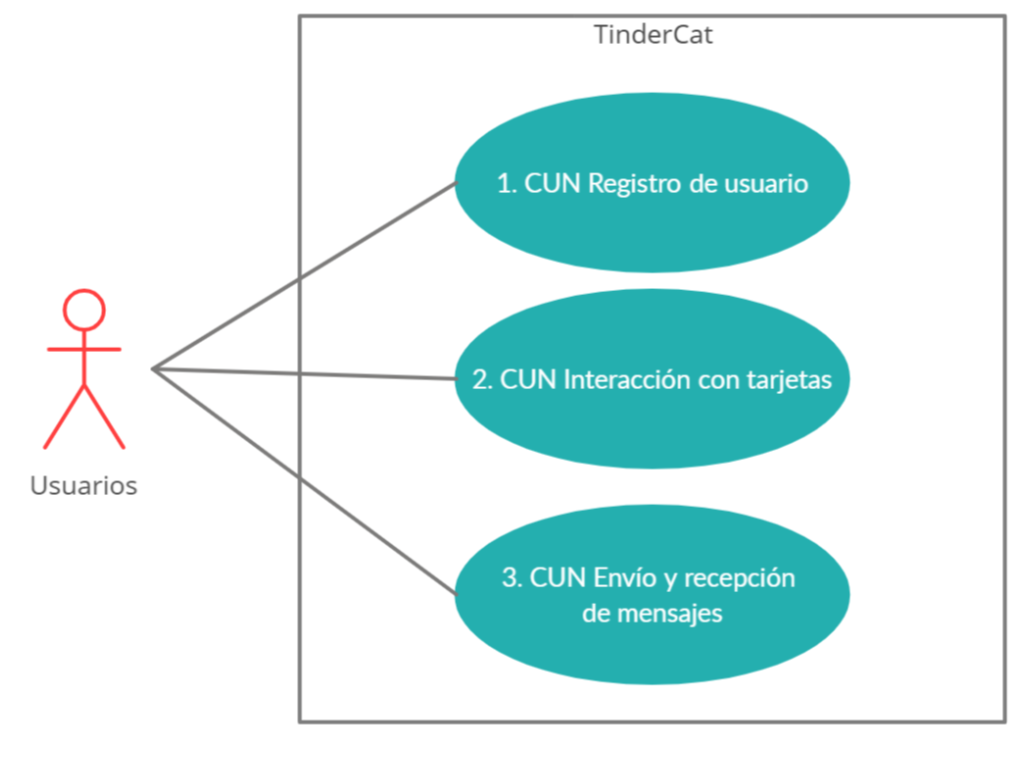
\includegraphics[width=\textwidth]{images/Caso de uso negocio.png}
        \caption{Caso de uso de negocio}
    \end{center}
\end{figure}    
\subsection{Reglas de negocios}
\begin{table}[h]
    \centering
    \resizebox{\textwidth}{!}{
    \begin{tabular}{| c | c | c |}
        \hline
        Número & Regla del Negocio & Descripción \\ \hline \hline
        1 & Condición de cliente & Todo pedido debe ser realizado por un cliente \\ \hline
        2 & Formas de pago & \parbox{10cm}{\centering Las formas de pago solo incluyen mediante \\ tarjeta de crédito o débito y por depósito en cuenta} \\ \hline
        3 & Formas de contacto & \parbox{10cm}{\centering Las únicas formas de contacto son mediante llamada telefónica y/o por Whatsapp} \\ \hline
        4 & Despacho de productos & \parbox{10cm}{\centering El personal de despacho solamente podrá ingresar a la puerta del domicilio si los productos son de gran volumen} \\ \hline
        5 & Envío de productos & \parbox{10cm}{\centering Los envíos y entrega de productos serán llevados a cabo cumpliendo las reglas de salubridad} \\ \hline
        6 & Devolución de productos & \parbox{10cm}{\centering En caso de envío a provincia, si el producto llega en mal estado, podrá solicitar un reembolso del pago o bien un reemplazo del producto} \\ \hline \hline
    \end{tabular}}
\end{table}

\clearpage
%--------------------------------------------------------------------------------
\section{Determinación del alcance}
Nuestra aplicación web debe llegar a facilitar la interacción a los usuarios, dueños de felinos, con otros que estén en un rango limitado de distancia asociada a su ubicación actual captura por la aplicación para mostrar tarjetas de vista como presentación de otros felinos que se adecuen a los parámetros de edad, raza y otros más establecidos por el usuario. Facilitando así la comunicación interna en la aplicación con usuarios con los cuales se haya hecho match.
\section{Requerimientos}
\subsection{Requerimientos Funcionales}
\begin{enumerate}
    \item El sistema debe permitir registrar un usuario nuevo.
    \item El sistema debe permitir loguear al usuario.
    \item El sistema debe recopilar nombre, edad, número de celular del usuario y la ubicación en tiempo real.
    \item El sistema debe recopilar información sobre su felino: nombre, fotos, raza, edad.
    \item El sistema debe mostrar tarjetas como presentación de otros felinos.
    \item El sistema debe permitir al usuario dar like o dislike a las tarjetas de presentación.
    \item El sistema debe hacer “match” con usuarios que se hayan dado mutuamente un like.
    \item El sistema debe unir en un chat interno a los usuarios que tengan “match”.
    \item El sistema debe permitir editar el perfil del usuario.
    \item El sistema debe permitir gestionar los felinos asociados a un usuario.
\end{enumerate}
\subsection{Requerimientos No Funcionales}
\begin{enumerate}
    \item El sistema debe validar el inicio de sesión
    \item El sistema debe solicitar una foto de perfil al usuario
    \item El sistema debe debe cerrar sesión en caso de estar inactivo por 10 minutos
    \item El sistema debe permitir reportar usuarios
    \item El sistema debe permitir desactivar o eliminar tu usuario
    \item El sistema debe tener una opción modo trabajo de fácil acceso
\end{enumerate}
\clearpage
%--------------------------------------------------------------------------------
\section{Descripción de Casos de Uso}
\subsection{Caso de Uso del Sistema General}
\begin{figure}[h]
    \begin{center}
        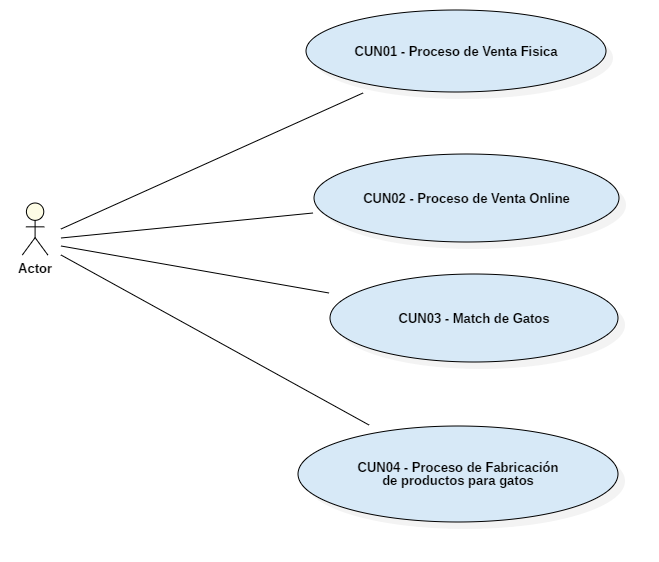
\includegraphics[width=0.5\textwidth]{images/Caso de uso general v2.png}
        \caption{caso de uso del sistema general}
    \end{center}
\end{figure}
\subsection{Descripción del Caso General}
La empresa está dedicada a la fabricación de productos para gatos, incluye también el proceso de venta al por mayor y menor de manera física o virtual.
El nuevo proceso es del sistema web que facilite a las personas dueños de gatos poder encontrar pareja a sus mascotas y les permita procrear. Este sistema almacenará información relevante personal y de contacto de los usuarios y mascotas para una buena comunicación entre dueños. Los información almacenada será tratada de forma segura según la ley N° 29733, Ley de Protección de Datos Personales.
\clearpage
%--------------------------------------------------------------------------------
\subsection{Caso de Uso de Sistema Específico CUN03}
\vspace{5mm}
\begin{figure}[h]
    \begin{center}
        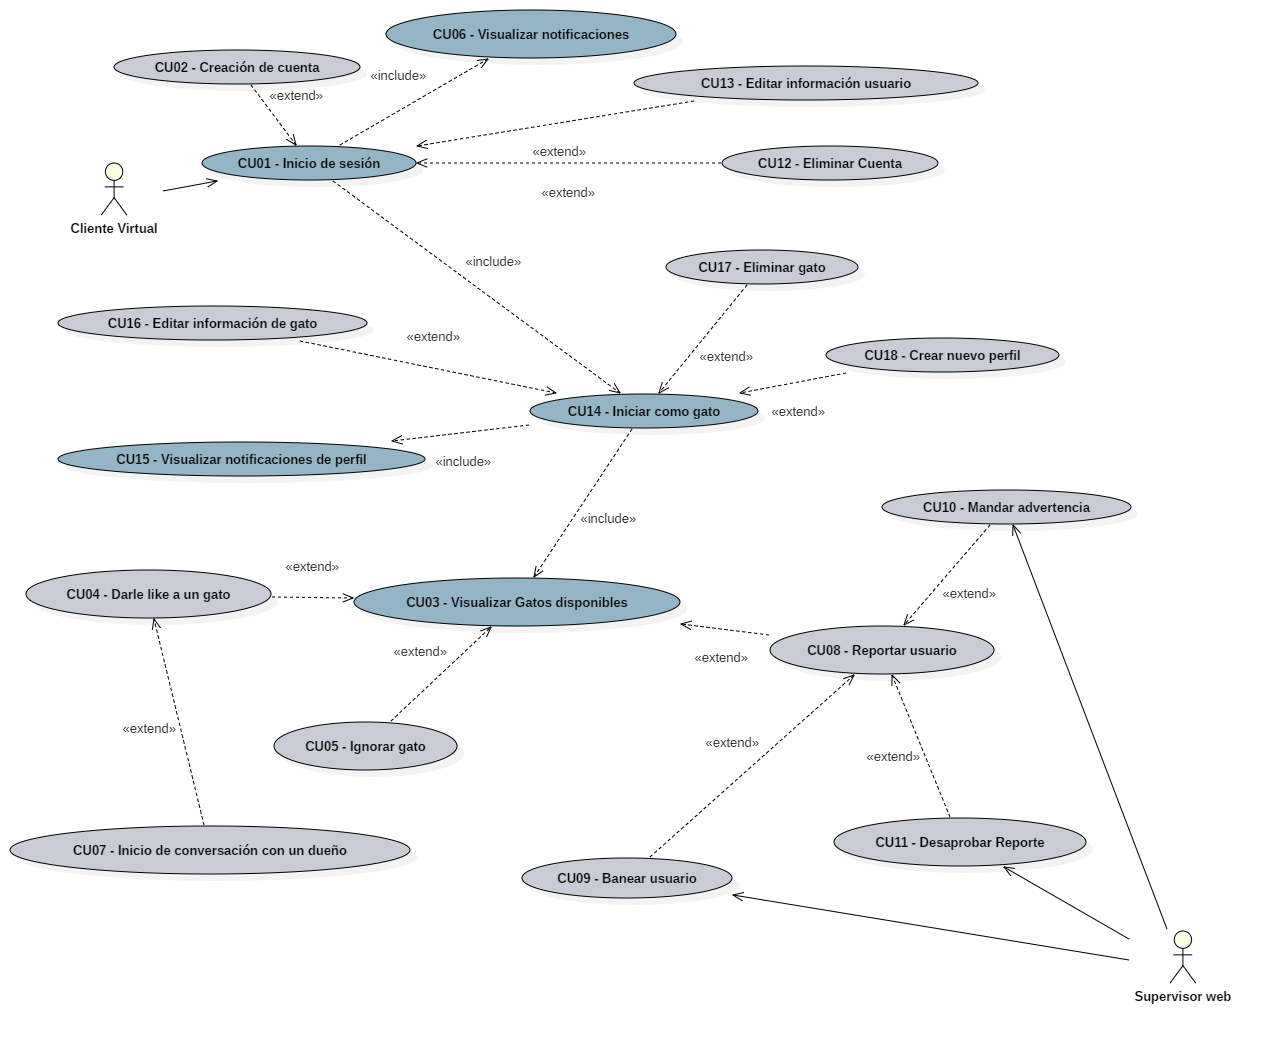
\includegraphics[width=\textwidth]{images/Caso de uso especifico.png}
        \caption{Caso de uso del sistema específico}
    \end{center}
\end{figure}
\subsection{Descripción del Caso Específico}
El sistema web para el emparejamiento de mascotas permitirá la creación de cuenta para los usuarios, una vez iniciado sesión se puede visualizar notificaciones tanto de usuario como de los perfiles de sus mascotas.
Este se brindará el servicio como un adicional al negocio además de la venta de sus productos. Se ofrecen varias funcionalidades similares a las que tienen las distintas aplicaciones de citas, además de ofrecer a un usuario tener muchos perfiles, uno para cada gato que tenga y estos se mantengan independientes.
\clearpage

%--------------------------------------------------------------------------------



\end{document}
